\documentclass[compress]{beamer}
%
% Choose how your presentation looks.
%
% For more themes, color themes and font themes, see:
% http://deic.uab.es/~iblanes/beamer_gallery/index_by_theme.html
%
\mode<presentation>
{
	\usetheme{Dresden}      % or try Darmstadt, Madrid, Warsaw, ...  
	%\useoutertheme{infolines} % split, tree, infolines
	%\useinnertheme{rectangles}
	\usecolortheme{orchid} % or try albatross, beaver, crane, ...
	\usefonttheme{structuresmallcapsserif}  % or try serif, structurebold, ...
	\setbeamertemplate{navigation symbols}{}
	\setbeamertemplate{caption}[numbered]
	\setbeamertemplate{footline}[frame number]
} 

\usepackage[english]{babel}
\usepackage[utf8x]{inputenc}
\usepackage{tikz}
\usetikzlibrary{trees,snakes,arrows}
\usepackage{tabularx}
\usepackage{subfig}
\usepackage{graphicx}
%\usepackage{animate}

\def\tobar{\mathrel{\mkern3mu  \vcenter{\hbox{$\scriptscriptstyle+$}}%
		\mkern-12mu{\to}}}

\usepackage{alphalph}
\renewcommand*{\thesubfigure}{%
	\alphalph{\value{subfigure}}%
}%

\title[BA Hobbhahn 2019]{Object Detection using the Scattering Transform}
\author{Marius Hobbhahn}
\date{\today}

\begin{document}
	
	\begin{frame}
		\titlepage
	\end{frame}
	%
	% Uncomment these lines for an automatically generated outline.
	%\begin{frame}{Outline}
	%  \tableofcontents
	%\end{frame}
	%
	\section{Introduction}
	\subsection{ } % for the dots - there most probably is a more elegant solution.
	%
	\begin{frame}{Motivation}
		\begin{block}{Problems}
			\begin{enumerate}
				\item Loads of data necessary for training
				\item Capability to generalize unclear for different circumstances (i.e. invariances w.r.t. translation, deformations, scale(?), rotation(?)
			\end{enumerate}
		\end{block}
		\begin{block}{Possible solutions}
			\begin{enumerate}
				\item Filters that generalize quickly
				\item Theoretical bounds for some invariances (translation) or Lipschitz continuity w.r.t deformations
			\end{enumerate}
		\end{block}
	\end{frame}
	%
	\begin{frame}{Scattering Transform}
		\begin{block}{Basic Idea}
			Static image filter that has certain theoretical guarantees with respect to invariances (i.e. location, scale, rotation).
		\end{block}
		\begin{equation}
		\psi(u) = C_1 (e^{iu.\xi} - C_2) e^{\frac{-|u|^2}{2\sigma^2}}
		\label{eq:morlet2d}
		\end{equation}
		\begin{figure}[!htb]
			\centering
			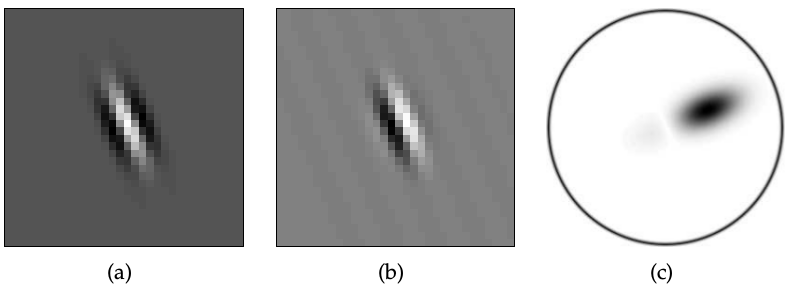
\includegraphics[width = 0.75\textwidth]{images/morlet2d.png}
			\caption{Complex morlet wavelet. a) Real part of $\psi$. b) Imaginary part of $\psi$. c) Fourier modulus $|\hat{\psi}|$.}
			\label{fig:morlet2d}
		\end{figure}
	\end{frame}
	%
	%what is U
	%what is f
	%what is \phi
	%what is S
	%what is \lambda
	%
	\begin{frame}{Visualization of the filter bank}
		\begin{figure}[!htb]
			\centering
			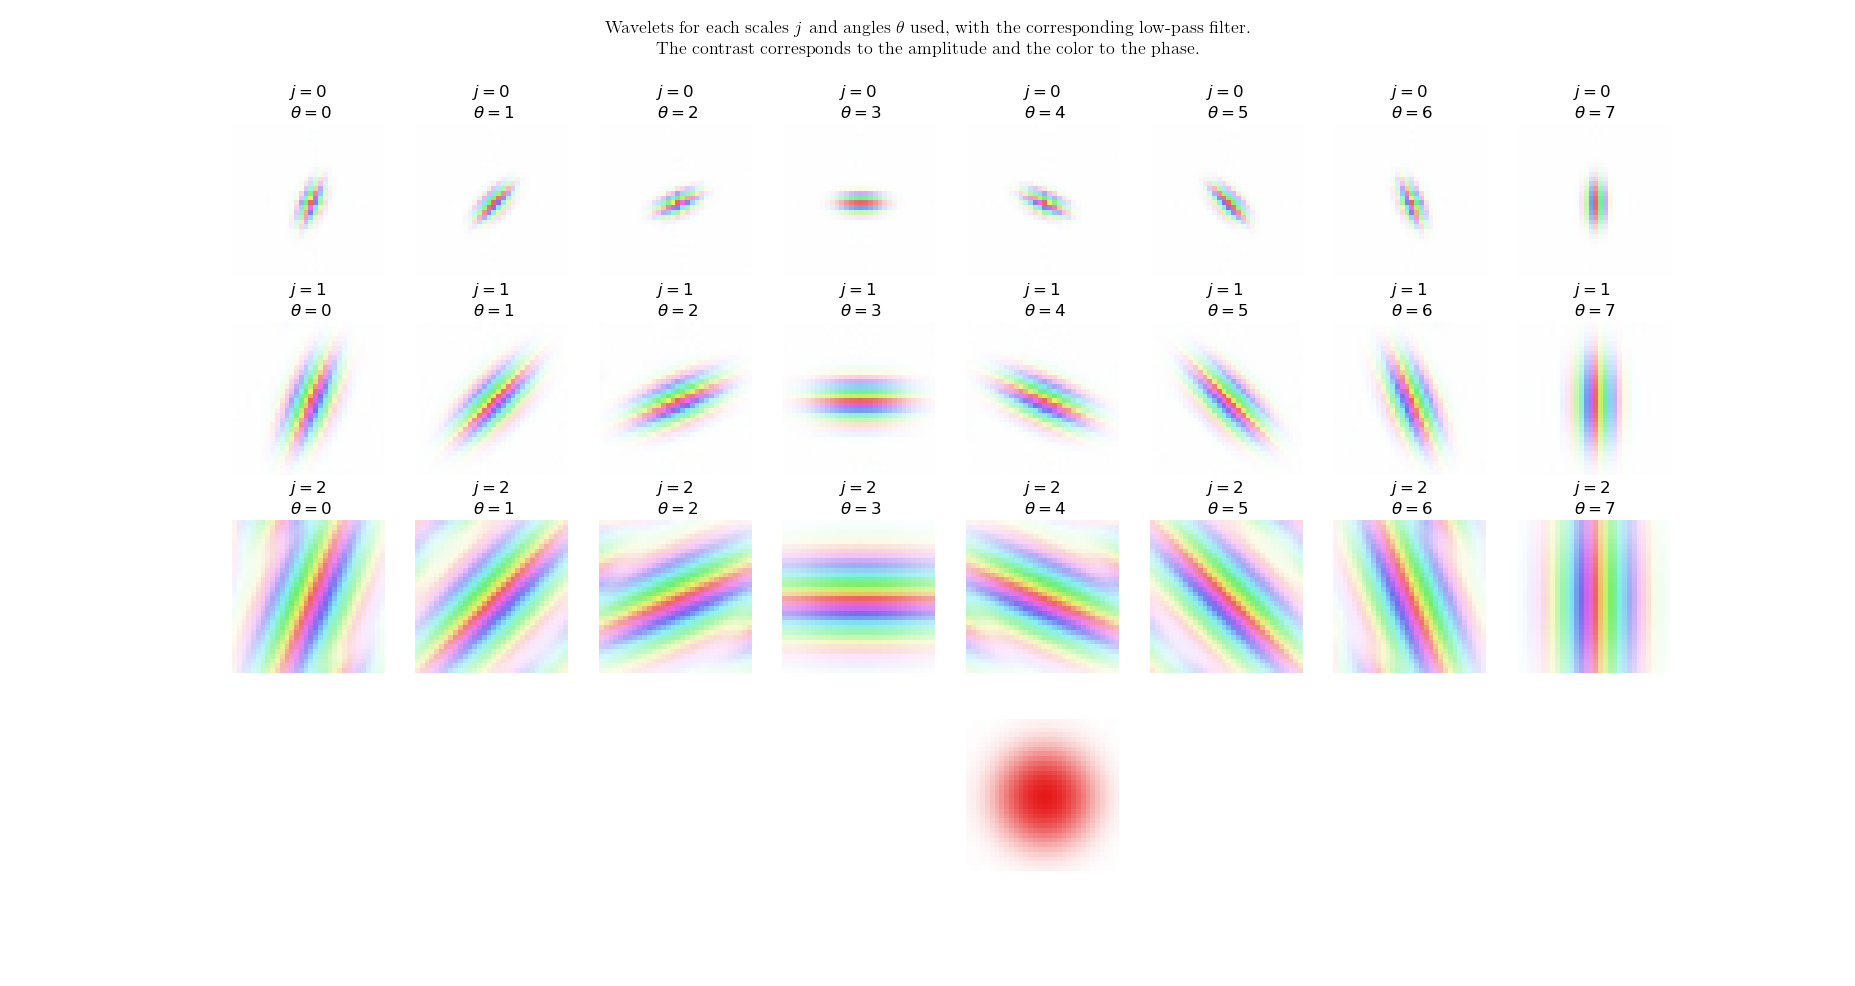
\includegraphics[width=\textwidth]{images/filter_bank_vis.png}
			\caption{Visualization of the filter bank}
			\label{fig:viz_filter_bank}
		\end{figure}
	\end{frame}
	%
	\begin{frame}{Scattering Networks}
		\begin{block}{Basic Idea}
			Apply the scattering transform multiple times to get higher order scattering coefficients.
		\end{block}
		\begin{figure}[!htb]
			\centering
			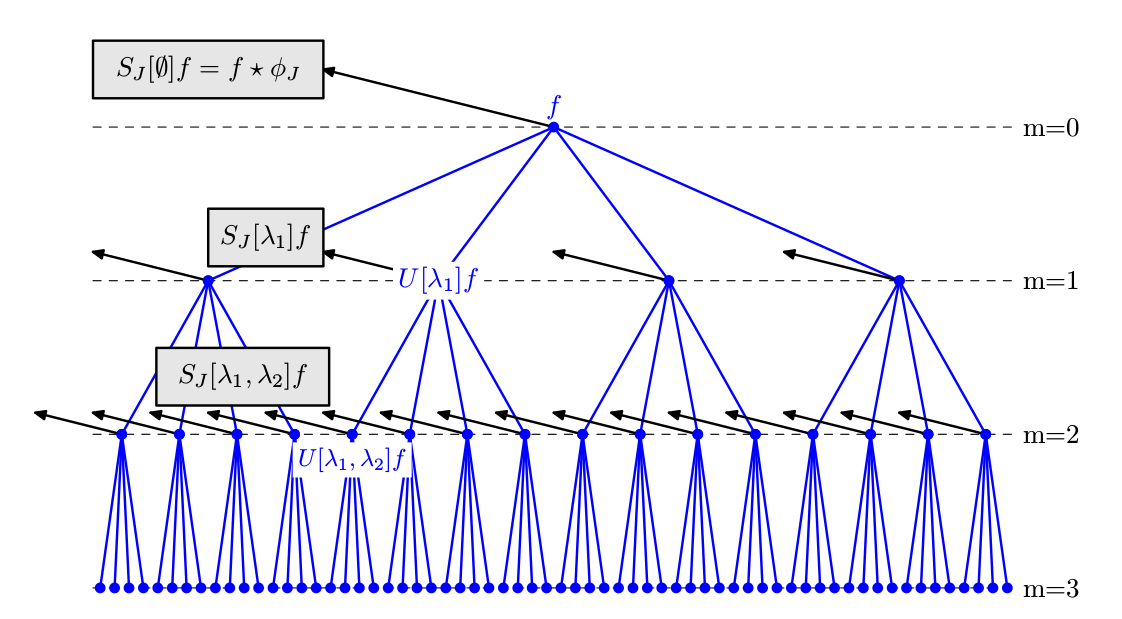
\includegraphics[width = 0.75\textwidth]{images/scattering_network.png}
			\caption{}
			\label{fig:scattering_network}
		\end{figure}
	\end{frame}
	%
	\begin{frame}{Example}
		\begin{equation}
		i \cdot (1 + JL) 
		\label{eq:order1_num_filters}
		\end{equation} 
		\begin{equation}
		i \cdot (1 + JL + \frac{1}{2}J(J-1)L^2)
		\label{eq:order2_num_filters}
		\end{equation}
		\begin{itemize}
			\item Let $J=2, L=8, N,M=32,32$ for a RGB image.
			\item number of outputs of the scattering network for $m=1$:
			$$ 3\cdot (1 + 2 * 8) = 51$$
			\item number of outputs of the scattering network for $m=2$:
			$$ 3 \cdot (1 + 16 + 0.5*2*1 * 64) = 243$$
			\item all outputs of size 8x8
		\end{itemize}
	\end{frame}
	%
	\begin{frame}{Hybrid scattering networks}
		\begin{figure}
			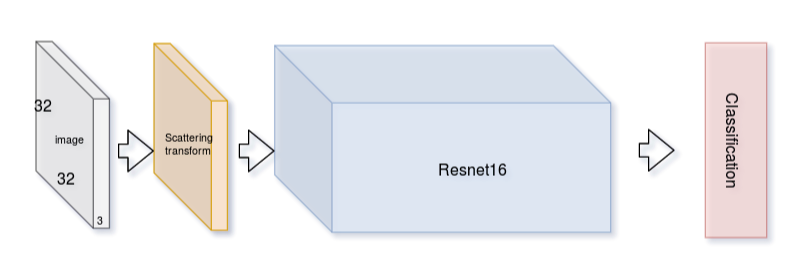
\includegraphics[width=0.9\textwidth]{images/arch_hybrid_scattering_CIFAR10.png}
			\caption{Architecture}
		\end{figure}
	\end{frame}
	%
	\section{Models/Experiments}
	\subsection{ } % for the dots - there most probably is a more elegant solution.
	\begin{frame}{Simple Single Shot MultiBox Detector (SSD)}
		\begin{figure}
			\centering
			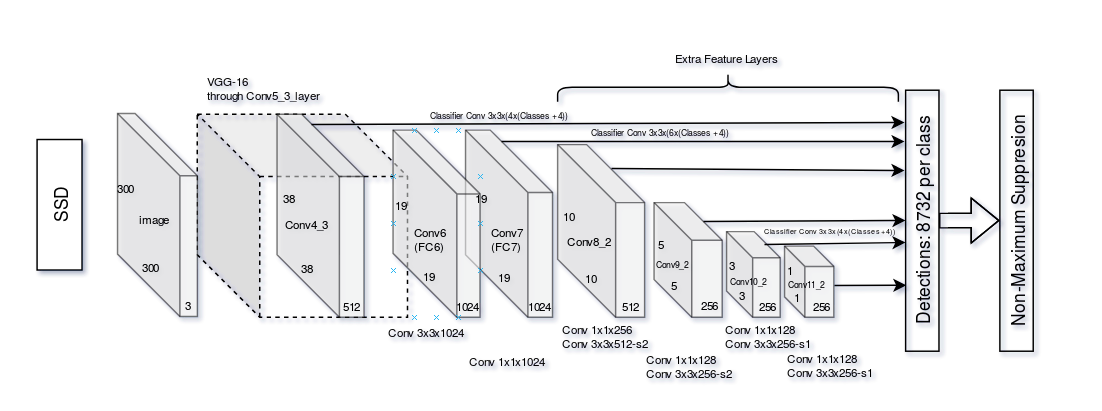
\includegraphics[width=\textwidth]{images/simple_ssd.png}
		\end{figure}
	\end{frame}
	%
	\begin{frame}{Sequential Scattering SSD}
		\begin{block}{}
			\begin{itemize}
				\item Scattering is applied before data is piped through SSD
			\end{itemize}
		\end{block}
		\begin{figure}
			\centering
			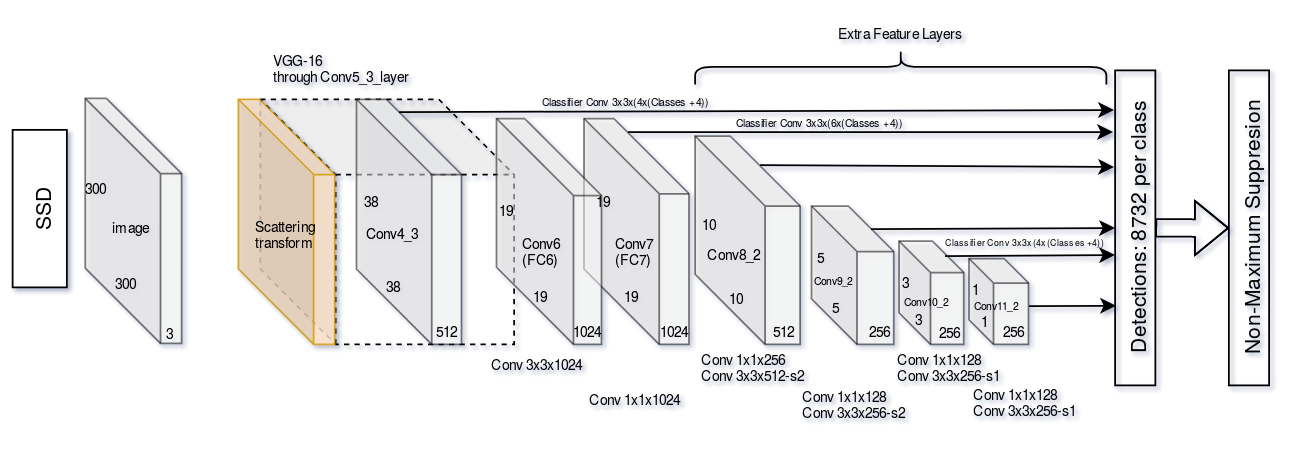
\includegraphics[width=\textwidth]{images/sequential_scattering_ssd.png}
		\end{figure}
	\end{frame}
	%
	\begin{frame}{Continuous Fusion Scattering SSD}
		\begin{block}{}
			\begin{itemize}
				\item Data is piped through scattering and standard SSD and continuously merged at different stages
			\end{itemize}
		\end{block}
		\begin{figure}
			\centering
			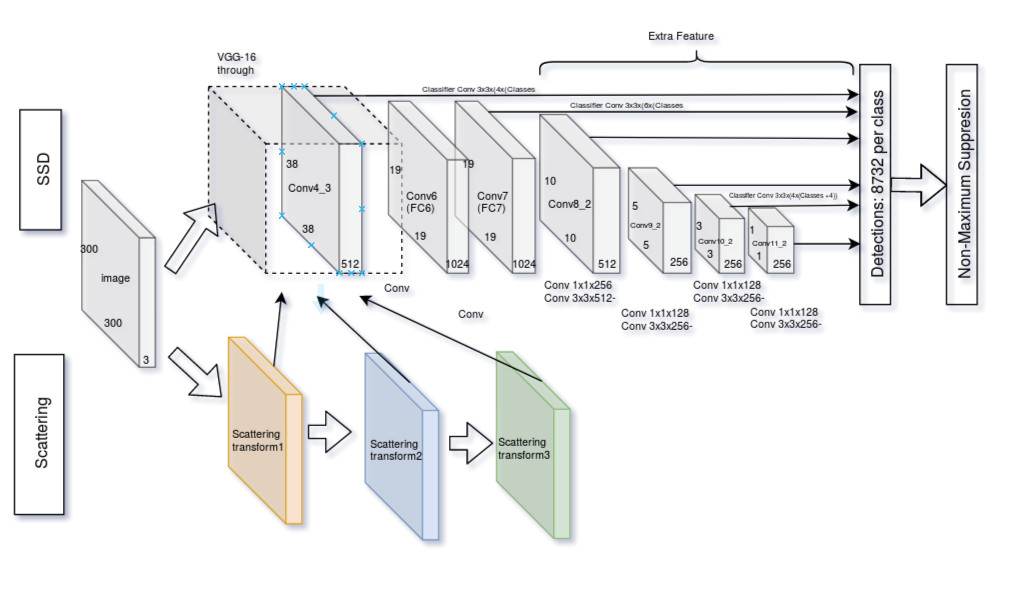
\includegraphics[width=0.8\textwidth]{images/parallel_scattering_ssd.png}
		\end{figure}
	\end{frame}
	%
	\begin{frame}{Status Quo}
		\begin{itemize}
			\item experimented with different hyperparameters and features for baseline SSD (pretrained, batch norm, augmentations, etc.) $\rightarrow$ still very bad results for kitti
			\item implemented sequential and parallel scattering $\rightarrow$ very high variance within the results
			\item created toy datasets to test invariances
		\end{itemize}
	\end{frame}
	%
	\begin{frame}{toy datasets}
		\begin{block}{Idea}
			Test if the promised invariants or continuities hold in empirical experiments
		\end{block}
		\begin{itemize}
			\item Transformation dataset
			\item Scale dataset
			\item Rotation dataset
			\item Deformation dataset
		\end{itemize}
	\end{frame}
	%
	\begin{frame}{Transformation dataset}
		\begin{figure}
			\centering
			\begin{tabular}{ccccc}
				\subfloat[]{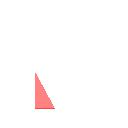
\includegraphics[width=2cm]{images/translation_examples/0000000_00.jpg}} 
				& \subfloat[]{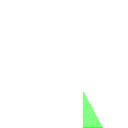
\includegraphics[width=2cm]{images/translation_examples/0000000_01.jpg}}&
				\subfloat[]{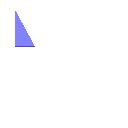
\includegraphics[width=2cm]{images/translation_examples/0000000_02.jpg}} &
				\subfloat[]{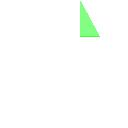
\includegraphics[width=2cm]{images/translation_examples/0000000_03.jpg}}&
				\subfloat[]{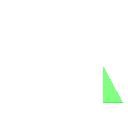
\includegraphics[width=2cm]{images/translation_examples/0000000_04.jpg}} \\
				\subfloat[]{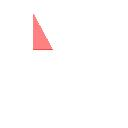
\includegraphics[width=2cm]{images/translation_examples/0000000_05.jpg}} 
				& \subfloat[]{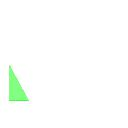
\includegraphics[width=2cm]{images/translation_examples/0000000_06.jpg}}&
				\subfloat[]{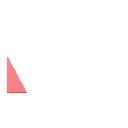
\includegraphics[width=2cm]{images/translation_examples/0000000_07.jpg}} &
				\subfloat[]{
\includegraphics[width=2cm]{images/translation_examples/0000000_08.jpg}}&
				\subfloat[]{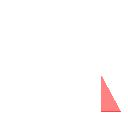
\includegraphics[width=2cm]{images/translation_examples/0000000_09.jpg}} 
			\end{tabular}
		\end{figure}
	\end{frame}
	%
	\begin{frame}{Scale dataset}
		\begin{figure}
			\centering
			\begin{tabular}{ccccc}
				\subfloat[]{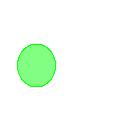
\includegraphics[width=2cm]{images/scale_examples/0000000_00.jpg}} 
				& \subfloat[]{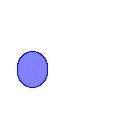
\includegraphics[width=2cm]{images/scale_examples/0000000_01.jpg}}&
				\subfloat[]{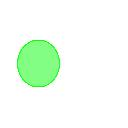
\includegraphics[width=2cm]{images/scale_examples/0000000_02.jpg}} &
				\subfloat[]{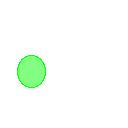
\includegraphics[width=2cm]{images/scale_examples/0000000_03.jpg}}&
				\subfloat[]{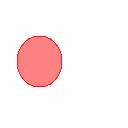
\includegraphics[width=2cm]{images/scale_examples/0000000_04.jpg}} \\
				\subfloat[]{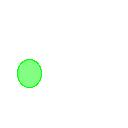
\includegraphics[width=2cm]{images/scale_examples/0000000_05.jpg}} 
				& \subfloat[]{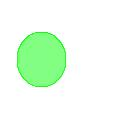
\includegraphics[width=2cm]{images/scale_examples/0000000_06.jpg}}&
				\subfloat[]{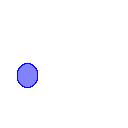
\includegraphics[width=2cm]{images/scale_examples/0000000_07.jpg}} &
				\subfloat[]{
\includegraphics[width=2cm]{images/scale_examples/0000000_08.jpg}}&
				\subfloat[]{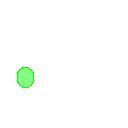
\includegraphics[width=2cm]{images/scale_examples/0000000_09.jpg}} 
			\end{tabular}
		\end{figure}
	\end{frame}
	%
	\begin{frame}{Rotation dataset}
		\begin{figure}
			\centering
			\begin{tabular}{ccccc}
				\subfloat[]{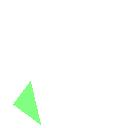
\includegraphics[width=2cm]{images/rotation_examples/0000003_00.jpg}} 
				& \subfloat[]{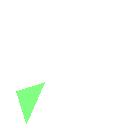
\includegraphics[width=2cm]{images/rotation_examples/0000003_01.jpg}}&
				\subfloat[]{
\includegraphics[width=2cm]{images/rotation_examples/0000003_02.jpg}} &
				\subfloat[]{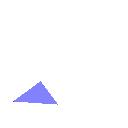
\includegraphics[width=2cm]{images/rotation_examples/0000003_03.jpg}}&
				\subfloat[]{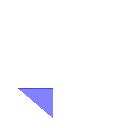
\includegraphics[width=2cm]{images/rotation_examples/0000003_04.jpg}} \\
				\subfloat[]{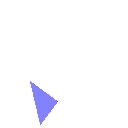
\includegraphics[width=2cm]{images/rotation_examples/0000003_05.jpg}} 
				& \subfloat[]{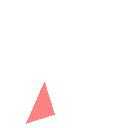
\includegraphics[width=2cm]{images/rotation_examples/0000003_06.jpg}}&
				\subfloat[]{
\includegraphics[width=2cm]{images/rotation_examples/0000003_07.jpg}} &
				\subfloat[]{
\includegraphics[width=2cm]{images/rotation_examples/0000003_08.jpg}}&
				\subfloat[]{
\includegraphics[width=2cm]{images/rotation_examples/0000003_09.jpg}} 
			\end{tabular}
		\end{figure}
	\end{frame}	
	%
	\begin{frame}{Deformation dataset}
		\begin{figure}
			\centering
			\begin{tabular}{ccccc}
				\subfloat[]{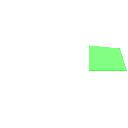
\includegraphics[width=2cm]{images/deformation_examples/0000001_00.jpg}} 
				& \subfloat[]{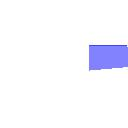
\includegraphics[width=2cm]{images/deformation_examples/0000001_01.jpg}}&
				\subfloat[]{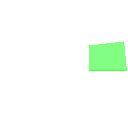
\includegraphics[width=2cm]{images/deformation_examples/0000001_02.jpg}} &
				\subfloat[]{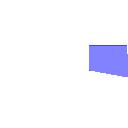
\includegraphics[width=2cm]{images/deformation_examples/0000001_03.jpg}}&
				\subfloat[]{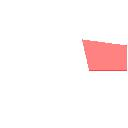
\includegraphics[width=2cm]{images/deformation_examples/0000001_04.jpg}} \\
				\subfloat[]{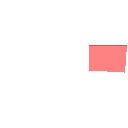
\includegraphics[width=2cm]{images/deformation_examples/0000001_05.jpg}} 
				& \subfloat[]{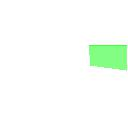
\includegraphics[width=2cm]{images/deformation_examples/0000001_06.jpg}}&
				\subfloat[]{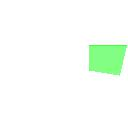
\includegraphics[width=2cm]{images/deformation_examples/0000001_07.jpg}} &
				\subfloat[]{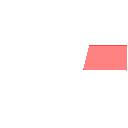
\includegraphics[width=2cm]{images/deformation_examples/0000001_08.jpg}}&
				\subfloat[]{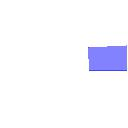
\includegraphics[width=2cm]{images/deformation_examples/0000001_09.jpg}} 
			\end{tabular}
		\end{figure}
	\end{frame}
	%
	\begin{frame}{Furthers plans and additional ideas}
		\begin{itemize}
			\item do baseline and scattering experiments on the currently existing datasets
			\item test pretrained and batch norm for scattering nets
			\item use other base-architecture: faster RCNN, masked RCNN, ...
			(trying to get the detectorch framework to run)
		\end{itemize}
	\end{frame}
	%
	\section{Outro}
	\subsection{ } % for the dots - there most probably is a more elegant solution.
	\begin{frame}{Questions and Suggestions}
		\begin{itemize}
			\item Any questions?
			\item Any suggestions, tips, ... are very welcome
		\end{itemize}
	\end{frame}
	%
	\begin{frame}[shrink=30]{References}
		\cite{scatteringTransform2012}, \cite{InvariantScatteringTextureDiscrimination2013}, \cite{DeepRotoTranslation2014}, 
		\cite{ScalingTheScatteringTransform2017},
		\cite{3DScatteringTransformNeuro2017}
		\bibliographystyle{alpha}
		\small\bibliography{bibliography}
	\end{frame}
	

\end{document}
